\documentclass[a4paper, 12pt]{article}
\usepackage[T2A,T1]{fontenc}
\usepackage[utf8]{inputenc}
\usepackage[english, russian]{babel}
\usepackage{graphicx}
\usepackage[hcentering, bindingoffset = 10mm, right = 15 mm, left = 15 mm, top=20mm, bottom = 20 mm]{geometry}
\usepackage{multirow}
\usepackage{lipsum}
\usepackage{amsmath, amstext}
\usepackage{siunitx}
\usepackage{subcaption}
\usepackage{wrapfig}
\usepackage{adjustbox}
\usepackage{enumerate, indentfirst, float}
\usepackage{capt-of, svg}
\usepackage{icomma}
\usepackage{wasysym}

\newenvironment{bottompar}{\par\vspace*{\fill}}{\clearpage}
 
\begin{document}
\begin{titlepage}

\newcommand{\HRule}{\rule{\linewidth}{0.5mm}} % Defines a new command for the horizontal lines, change thickness here

\center % Center everything on the page
 
%----------------------------------------------------------------------------------------
%	HEADING SECTIONS
%----------------------------------------------------------------------------------------

\textsc{\LARGE Московский Физико-Технический Институт}\\[1,5cm] % Name of your university/college
\textsc{\Large Кафедра общей физики}\\[0.5cm] % Major heading such as course name
\textsc{\large Вопрос по выбору}\\[0.5cm] % Minor heading such as course title

%----------------------------------------------------------------------------------------
%	TITLE SECTION
%----------------------------------------------------------------------------------------

\HRule
\\[0.4cm]
{ \huge \bfseries  Измерение удельного сопротивления воздуха}
\\[0.2cm] % Title of your document
\HRule
\\[1.5cm]


 
%----------------------------------------------------------------------------------------
%	AUTHOR SECTION
%----------------------------------------------------------------------------------------


\begin{flushleft} \large
	\emph{Автор:}\\
	Ушаков Роман \\
	513 группа
\end{flushleft}


\begin{bottompar}
	\begin{center}
		
\includegraphics[width = 80 mm]{logo.jpg}
	\end{center}
	{\large \today}

\end{bottompar}
\vfill % Fill the rest of the page with whitespace

\end{titlepage}

\subsection*{Цель работы}
Измерение удельного сопротивления воздуха.

\subsection*{Необходимое оборудование}
Линейка, карандаш, нить, два шарика для настольного тенниса, секундомер, любой резиновый или пластиковый предмет, который удобно электризовать (в данной работе выбран воздушный шарик <<ФАКИ>>).

\subsection*{Теоретический материал}

Заряд уединенного заряженного шарика, подвешенного на тонкой нити в воздухе, с течением времени уменьшается. Это связано с конечной величиной удельного сопротивления воздуха $\rho$. Запишем закон Ома в дифференциальной форме:

\begin{equation}
\vec{j} = \lambda \vec{E}
\end{equation}

Учитывая соотношение $\lambda = \dfrac{1}{\rho}$, получим в итоге:

\begin{equation}
\vec{j} = \frac{1}{\rho}\vec{E}
\end{equation}

Теперь найдём величину всего тока $I$. Он равен:

\begin{equation}
I = \oiint_S j dS = \frac{1}{\rho}\oiint_S E dS = \dfrac{4 \pi q}{\rho}
\end{equation}

В последнем равенстве применена теорема Гаусса : $\oiint_S E dS = 4 \pi q$. Учитывая, что $I = -\dfrac{dq}{dt}$, получаем дифференциальное уравнение:

\begin{equation}
\frac{dq}{dt} = - \frac{q}{\rho \varepsilon_0}
\end{equation}

Уравнение записано в СИ. Решением этого дифференциального уравнения является функция $q(t) = q_0  e^{-\frac{t}{\tau}}$, где $q_0$~---
~начальный заряд шарика, $\tau = \varepsilon_0 \rho$~---~время, за которое заряд мячика уменьшается в $e$ раз. 
\begin{equation}
\frac{dq}{dt} = - \frac{q}{\rho \varepsilon_0}
\end{equation}

Тогда $\rho$ выражается:
\begin{equation}
\rho = \frac{T_{1/2}}{\varepsilon_0 \cdot ln 2}
\end{equation}

Заметим, что закон Кулона взаимодействия двух точечных зарядов неприменим в данных условиях из-за перераспределения индуцированных на шариках зарядов.

\begin {figure}[H]
\begin{center}
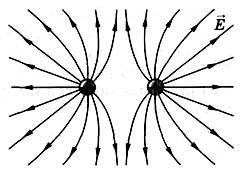
\includegraphics[width=0.6\textwidth]{7}
\end{center}
\end {figure}

\subsection*{Экспериментальная установка}

Параметры установки:

\begin{equation}
\begin{aligned}
L=140 \text{ см } \\
d_0=40 \text{ мм}
\end{aligned}
\end{equation}


\begin{figure}[h]
\begin{center}
\begin{minipage}[h]{0.45 \linewidth}
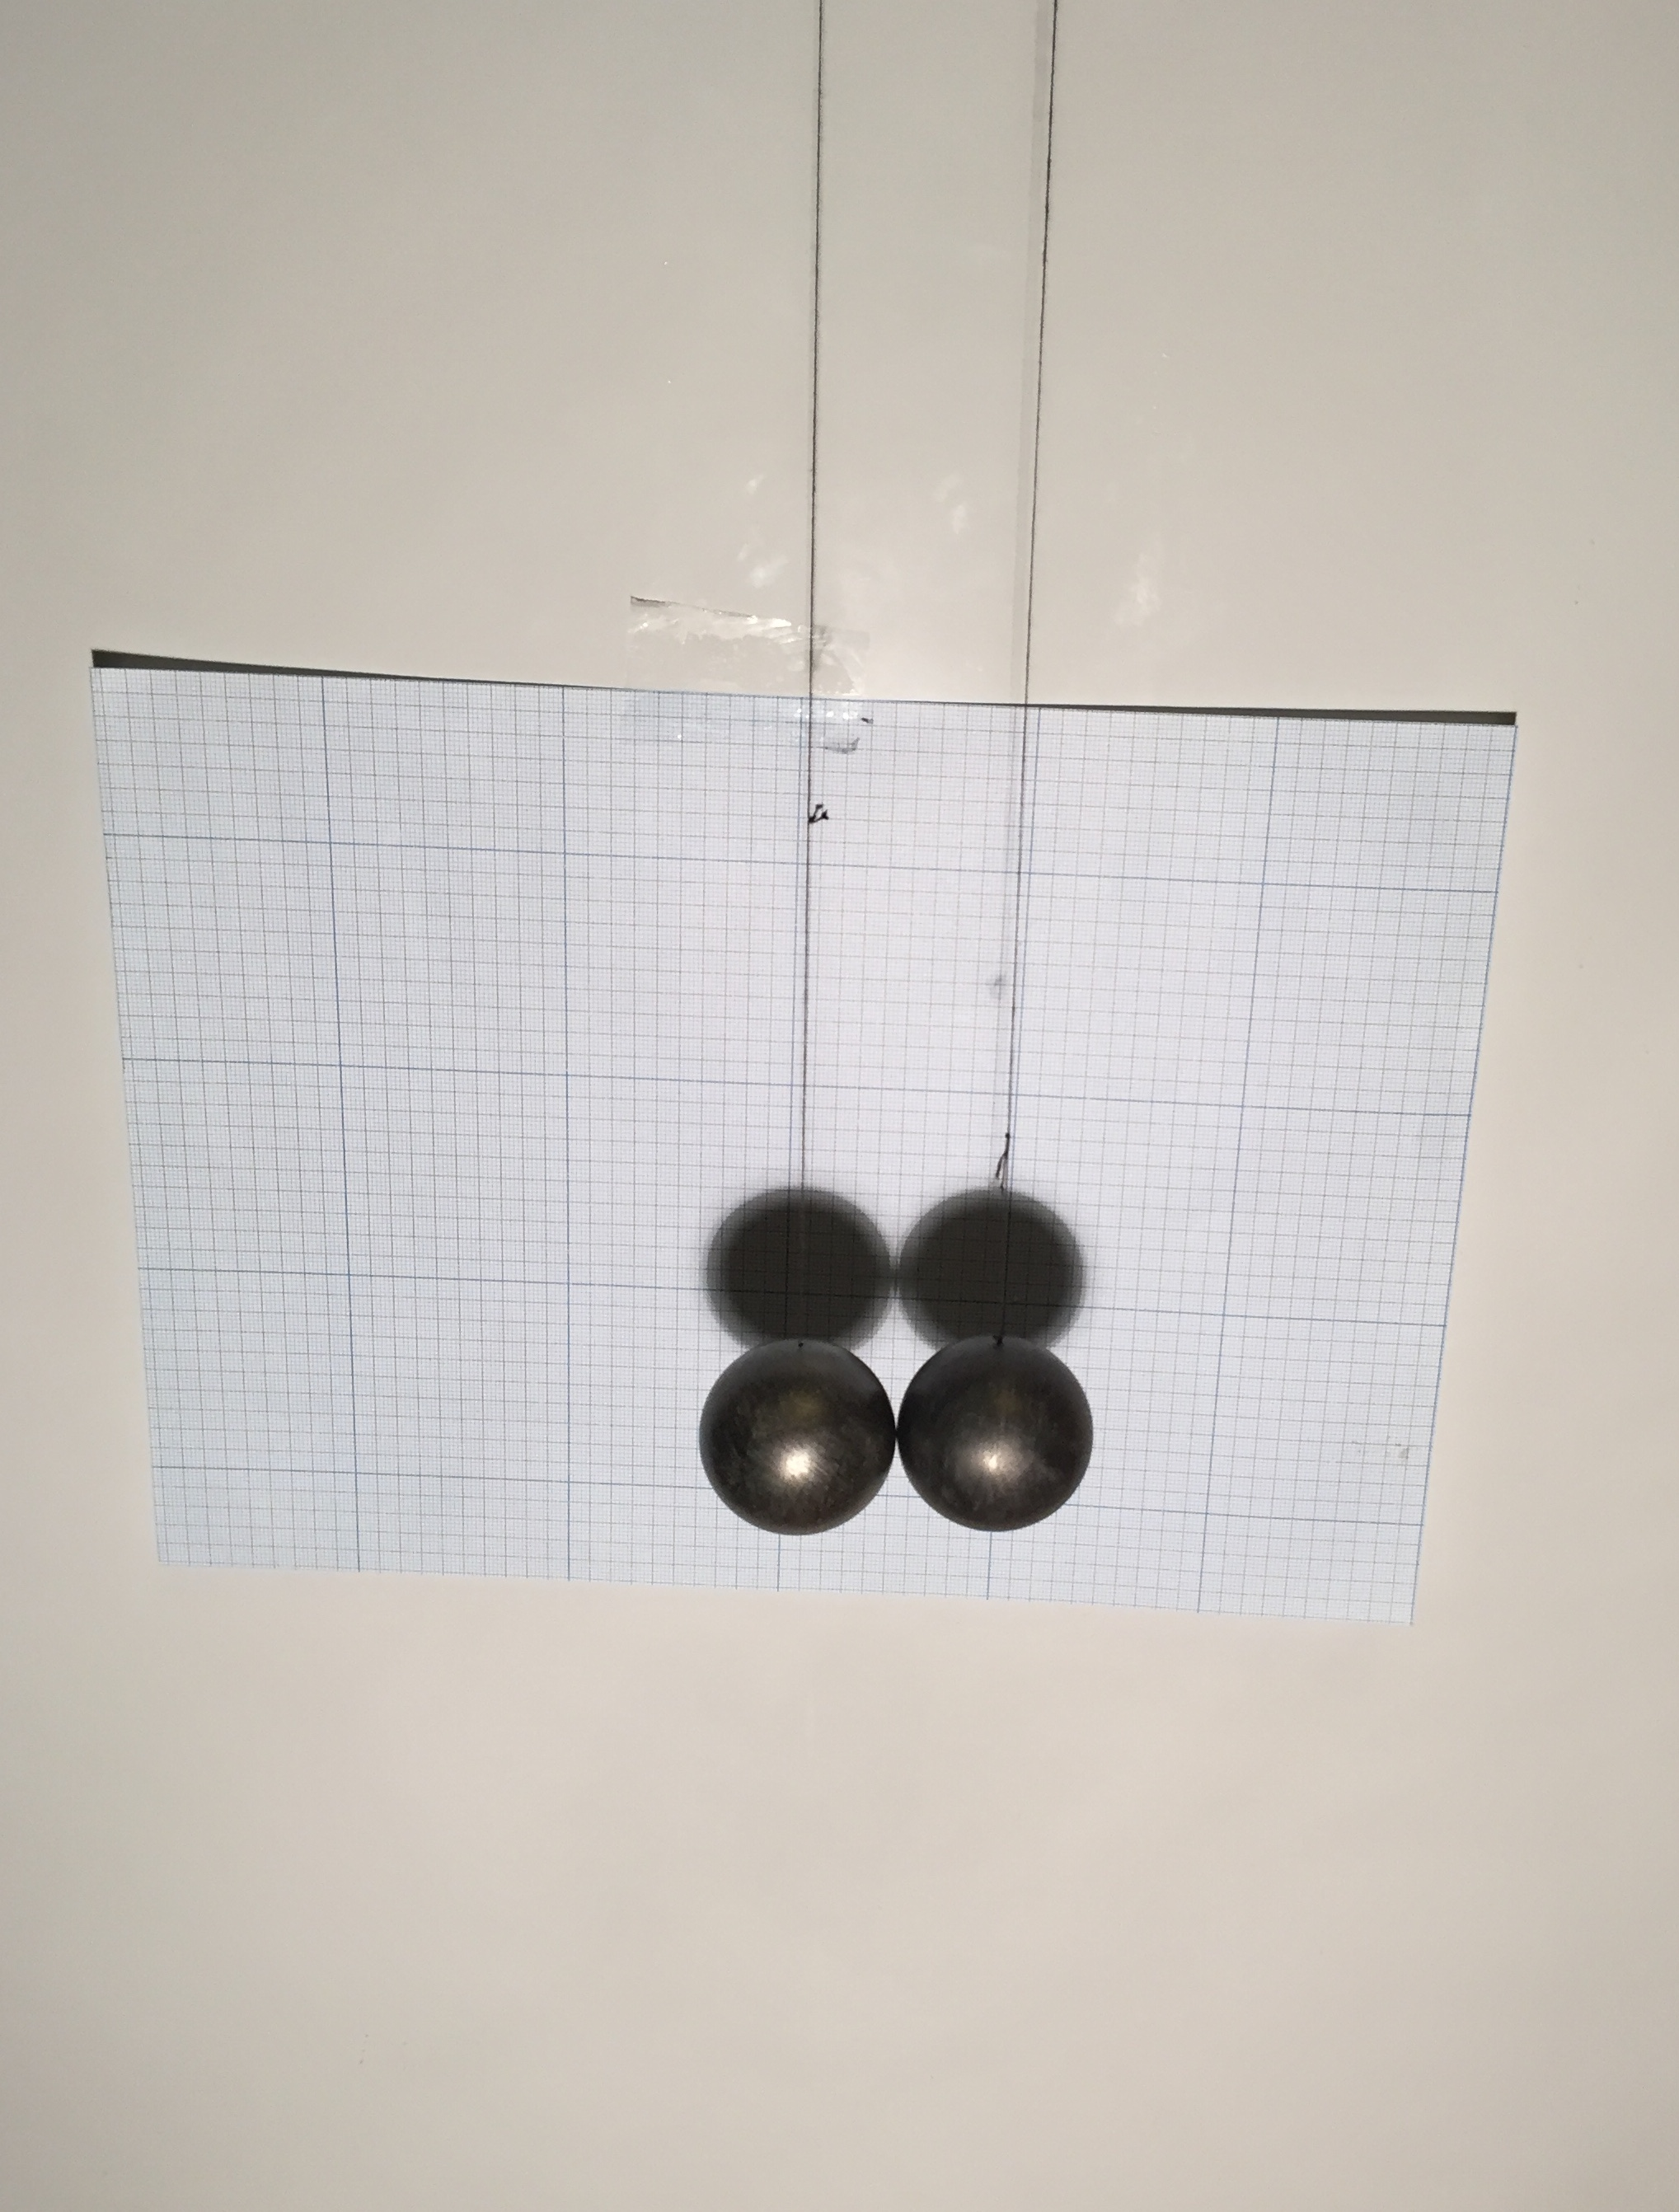
\includegraphics[height=10cm]{3}
\end{minipage}
\hfill 
\begin{minipage}[h]{0.45 \linewidth}
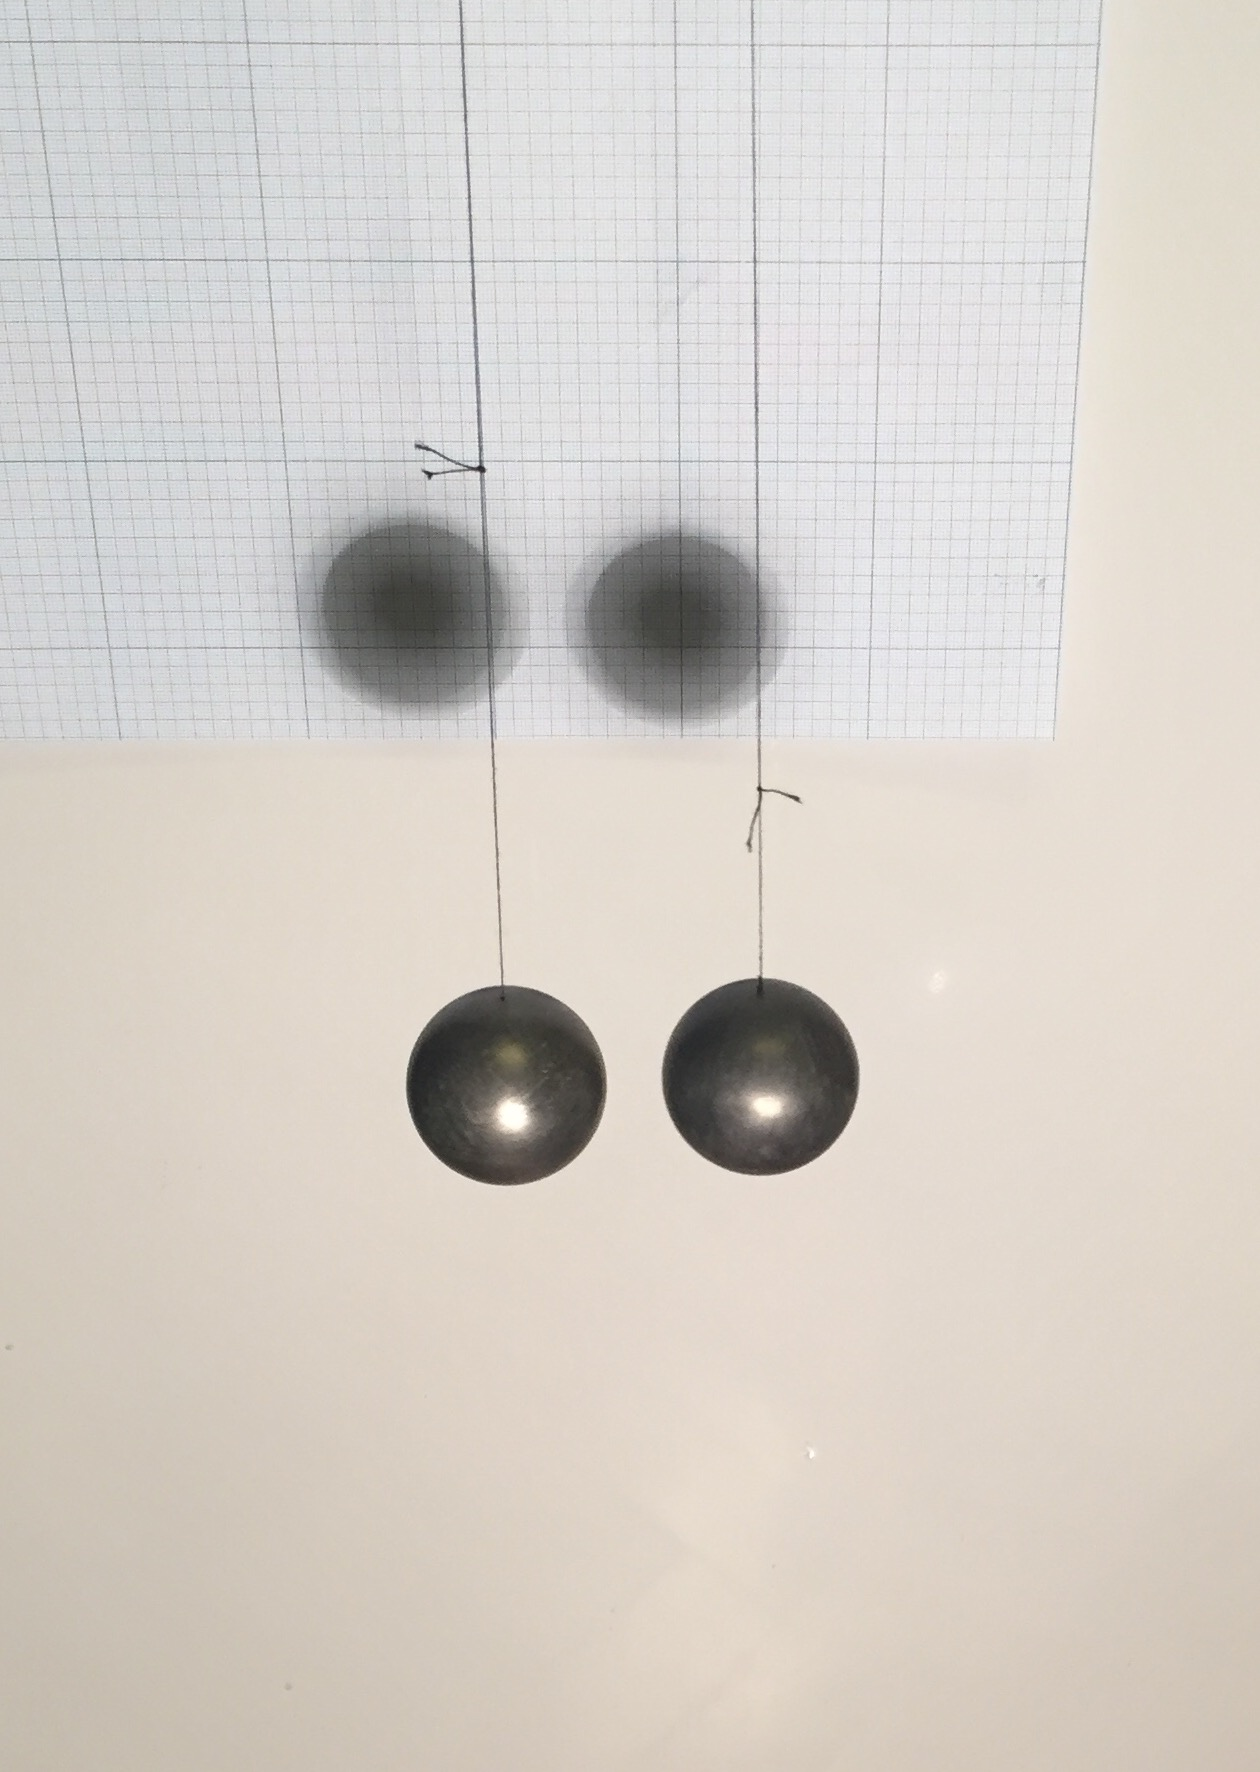
\includegraphics[height=10cm]{5}
\end{minipage}
\end{center}
\end{figure}


\subsection*{Ход работы}

\begin{figure}[H]
\begin{center}
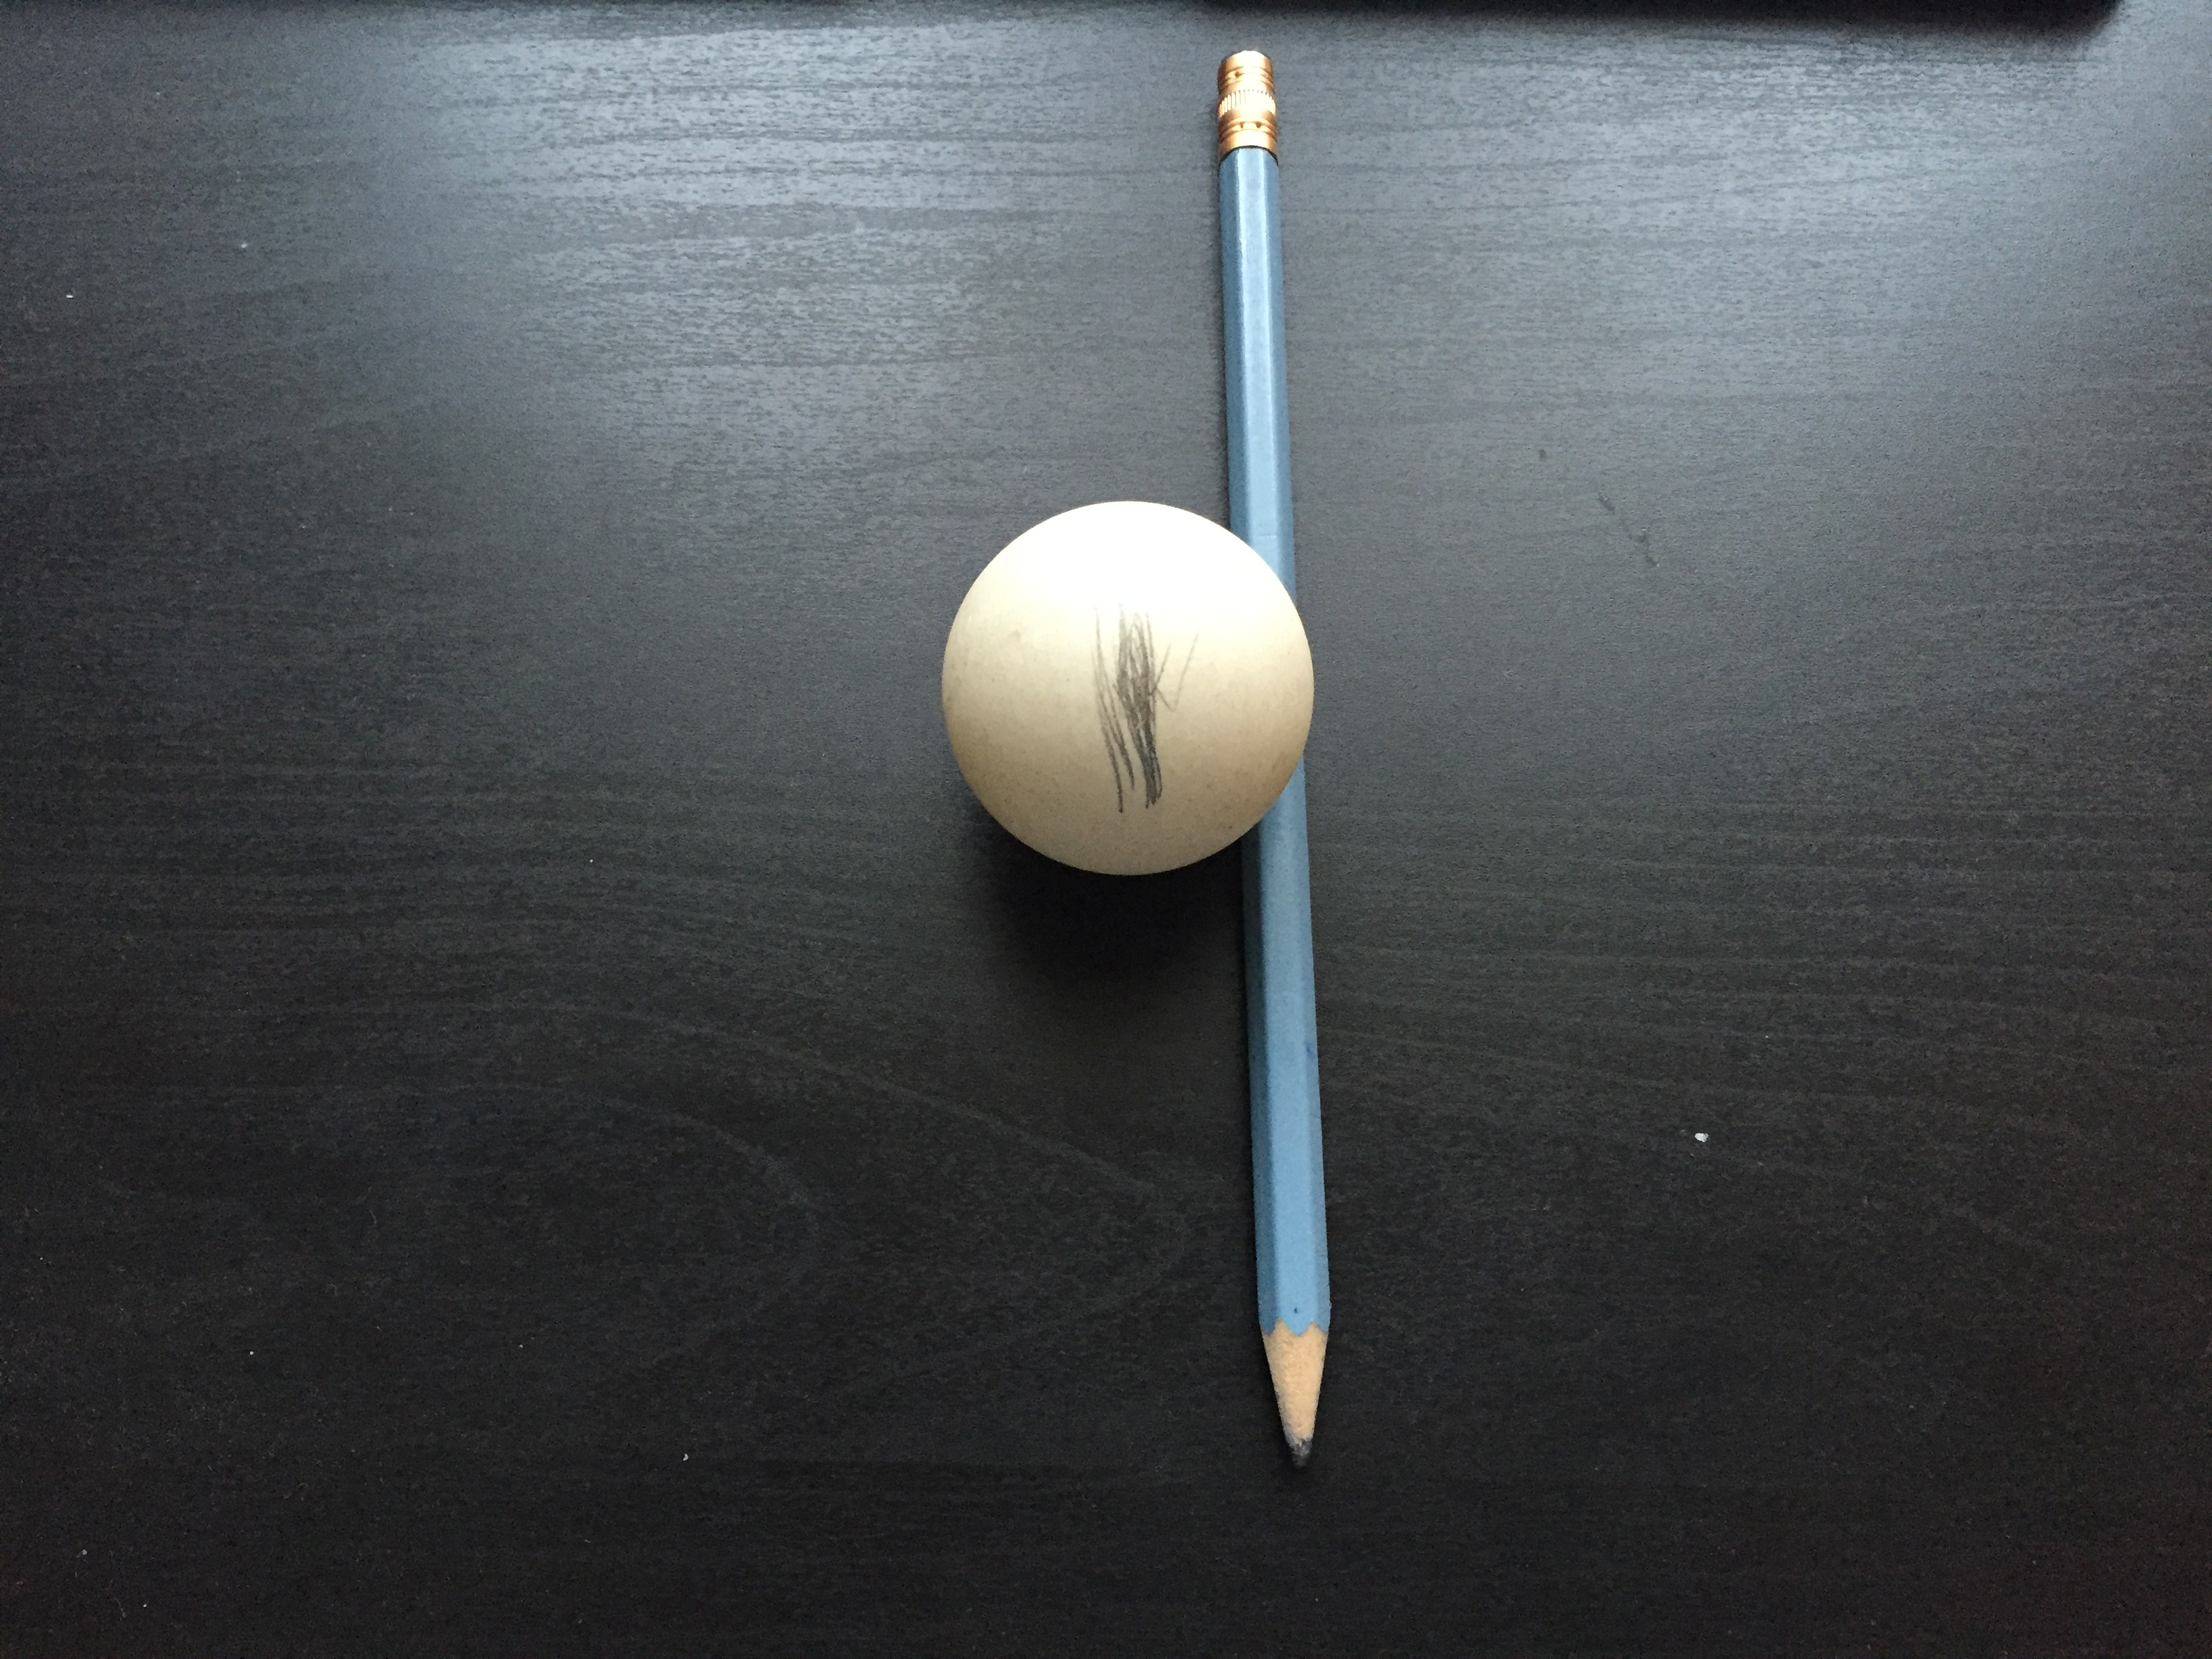
\includegraphics[width=0.6\textwidth]{4}
\end{center}
\end{figure}


Закрасим теннисные шарики карандашом, затем подвесим их так, чтобы расстояние между нитями равнялось диаметру шарика $d_0=2R=40$ мм. Длина нитей $L=140$ cм. Незаряженные шарики при этом слегка соприкасаются. С помощью линейки будем измерять расстояние между шариками.

\subsection*{Калибровка установки}

Заряжаем теннисные мячики с помощью воздушного шарика «ФАКИ». Измеряем расстояние между нитями на высоте 10 см от шариков. Полученное расстояние около $d_1=70$ мм. Затем разряжаем один из шариков, касаясь его рукой. После соприкосновения между собой шарики снова расходятся, но на этот раз на расстояние около $d_2=40$  мм. Заряды шариков при этом уменьшаются вдвое. Калибровка проведена.

Вновь заряжаем шарики так, что расстояние между нитями, отсчитанное по линейке, было $d_1=75$ мм. С помощью секундомера измеряем время $T_{\frac{1}{2}}$ , за которое расстояние между нитями уменьшается до $d_2 = 45$ мм. Это время соответствует уменьшению заряда вдвое.


\subsection*{Измерения}

I серия опытов: $d_1 = 73$ мм, $d_0 = 41$ мм

\vspace{0.5cm}

\begin{tabular}{|c|r|r|r|r|r|r|r|r|r|}
\hline
номер опыта & 1 & 2 & 3 & 4 & 5 & 6 & 7 & 8 & 9 \\
\hline
$T_{\frac{1}{2}}$, с & 468 & 471 & 474 & 490 & 463 & 453 & 448 & 501 & 451 \\
\hline
$\rho$, Ом $\cdot$ м $\cdot 10 ^{13}$ & 7.6 & 7.6 & 7.7 & 8.0 & 7.5 & 7.4 & 7.3 & 8.2 & 7.4\\
\hline
\end{tabular}

\vspace{1.5cm}

II серия опытов: $d_1 = 78$ мм, $d_0 = 43$ мм

\vspace{0.5cm}

\begin{tabular}{|c|r|r|r|r|r|r|r|r|r|r|}
\hline
номер опыта & 1 & 2 & 3 & 4 & 5 & 6 & 7 & 8 & 9 \\
\hline
$T_{\frac{1}{2}}$, с & 498 & 546  & 489 & 462 & 473 & 476 & 489 & 457 & 486  \\
\hline
$\rho$, Ом $\cdot$ м $\cdot 10 ^{13}$ & 8.1 & 8.9 & 8.0 & 7.5 & 7.7 & 7.8 & 8.0 & 7.5 & 8.0\\
\hline
\end{tabular}

\vspace{1.5cm}

III серия опытов: $d_1 = 76$ мм, $d_0 = 42$ мм

\vspace{0.5cm}

\begin{tabular}{|c|r|r|r|r|r|r|r|r|r|r|}
\hline
номер опыта & 1 & 2 & 3 & 4 & 5 & 6 & 7 \\
\hline
$T_{\frac{1}{2}}$, с & 475  & 467 & 474 & 497  & 435 & 449 & 478  \\
\hline
$\rho$, Ом $\cdot$ м $\cdot 10 ^{13}$ & 7.8 & 7.6 & 7.7 & 8.1 & 7.0  & 7.3 & 7.8\\
\hline
\end{tabular}

\vspace{1cm}

Полученные в результате опыта значения:
$$ \rho = 7.7 \cdot 10^{13} \text{ Ом $\cdot$ м, } \sigma_{T_{1/2}} = 23 \text{ c, } \sigma_{\rho} = 0.4\cdot 10^{13} \text{ Ом $\cdot$ м} \rightarrow \rho = (7.7 \pm 0.4) \cdot 10^{13} \text{ Ом $\cdot$ м} $$



Реальное значение удельного сопротивления воздуха зависит  от температуры и влажности и колеблется в диапазонах $\rho = 10^{13} - 10^{15}$ Ом $\cdot$ м. 

\subsection*{Вывод}

В данной работе был продемонстрирован способ измерения удельного сопротивления воздуха. Однако данный способ применим не только к воздуху, но и к любым средам, в которых выполняется закон Ома. Важно заметить, что в построении теории мы не использовали закон Кулона, так как заряженные шарики нельзя считать точечными зарядами: поверхностные заряды перераспределяются и имеют сложную конфигурацию. 

\subsection*{Источники}

[1] \textit{Общий курс физики. Электричество. Д. В. Сивухин} 

[2] \textit{International Physics Olympiad 2015}


\end{document}